\documentclass[a4]{article}

\usepackage{tikz}
\usepackage[a4paper, margin=5mm]{geometry}
\usepackage{relsize}

\usetikzlibrary[positioning]

\newcommand{\width}{6}
\newcommand{\height}{9}
\newcommand{\margin}{0.5}

\newcommand{\beername}{Black Hole Son}
\newcommand{\beerstyle}{Imperial stout}
\newcommand{\abv}{8.40\%}
\newcommand{\bottledate}{01-02-2020}

\begin{document}

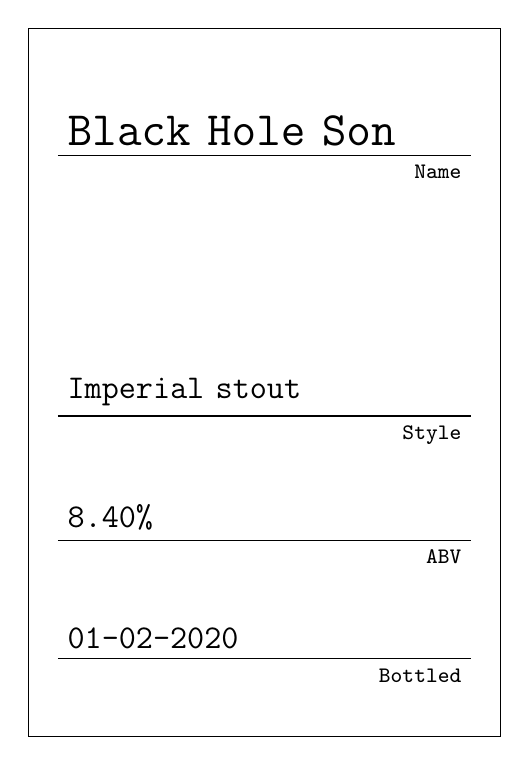
\begin{tikzpicture}

\tikzstyle{beerlabel}=[rectangle, draw, minimum width=6cm, minimum height=9cm]
\tikzstyle{namelabel}=[text width=5cm, font=\LARGE\ttfamily]
\tikzstyle{valuelabel}=[text width=5cm, font=\large\ttfamily]
\tikzstyle{label}=[text width=5cm, align=right, font=\footnotesize\ttfamily]

\node [beerlabel] (label) at (0,0) {};

\node [namelabel] (name) [below = of label.north] {\beername};
\draw (name.south west) -- (name.south east);
\node [label] (namelabel) [below = 0 of name] {Name};

\node [valuelabel] (bottledate) [above = 1cm of label.south] {\bottledate};
\draw (bottledate.south west) -- (bottledate.south east);
\node [label] (bottledlabel) [below = 0 of bottledate] {Bottled};

\node [valuelabel] (abv) [above = 1cm of bottledate] {\abv};
\draw (abv.south west) -- (abv.south east);
\node [label] (abvlabel) [below = 0 of abv] {ABV};

\node [valuelabel] (style) [above = 1cm of abv] {\beerstyle};
\draw (style.south west) -- (style.south east);
\node [label] (stylelabel) [below = 0 of style] {Style};

\end{tikzpicture}

\end{document}
